\chapter{Manuel utilisateur}

\section{Généralités}
\subsection{Introduction}

Cette section constitue le manuel utilisateur du projet BAGOmaze. Il explique comment naviguer dans les différents menus, configurer le jeu et se déplacer dans le labyrinthe.

\subsection{Arborescence des interfaces}
\dirtree{%
	.1 Main menu\DTcomment{Menu principal}.
		.2 Play\DTcomment{Menu de choix du mode de jeu}.
			.3 Arcade\DTcomment{Mode de jeu "time attack"}.
			.3 Choose level\DTcomment{Choix d'un niveau statique}.
				.4 Level 1.
				.4 Level 2.
				.4 Level 3.
				.4 Level 4.
				.4 Level 5.
			.3 Random\DTcomment{Génération aléatoire d'un niveau}.
		.2 Configure\DTcomment{Configuration de l'application}.
}



\section{Lancement du jeu}

Il est préférable de lancer le jeu à partir d'un terminal. Pour ce faire, ouvrir un terminal et se positionner dans le dossier contenant l'exécutable du jeu.

Pour lancer le jeu, exécuter la commande :
\begin{Verbatim}
	./BAGOmaze
\end{Verbatim}

Le jeu se lance en prenant la totalité de l'espace sur le terminal. Le menu principal de l'application apparaît.


\section{Menu principal}

\begin{center}
	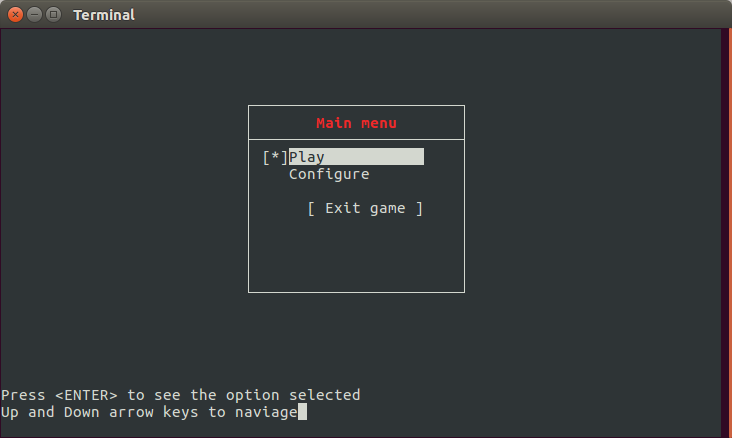
\includegraphics[width=0.75\textwidth]{annexe-manuel_utilisateur/rsrc/Main_Menu.png}
\end{center}

Le menu principal présente trois options :
\begin{itemize}
	\item \textbf{Play :} Permet d'accéder à l'écran de choix du mode de jeu.
	\item \textbf{Configure :} Permet d'accéder à l'écran de configuration du jeu.
	\item \textbf{Exit game :} Permet de quitter le jeu.
\end{itemize}

\paragraph{Nota :} L'écran de configuration n'est actuellement pas implémenté.

\paragraph{} L'opérateur peut naviguer entre les options en utilisant les touches directionnelles de son clavier pour mettre en surbrillance l'entrée du menu qu'il souhaite sélectionner. \\
Pour activer l'entrée du menu actuellement surlignée, l'opérateur doit presser la touche "Entrée" de son clavier.


\section{Menu "Play" - Choix du mode de jeu}

\begin{center}
	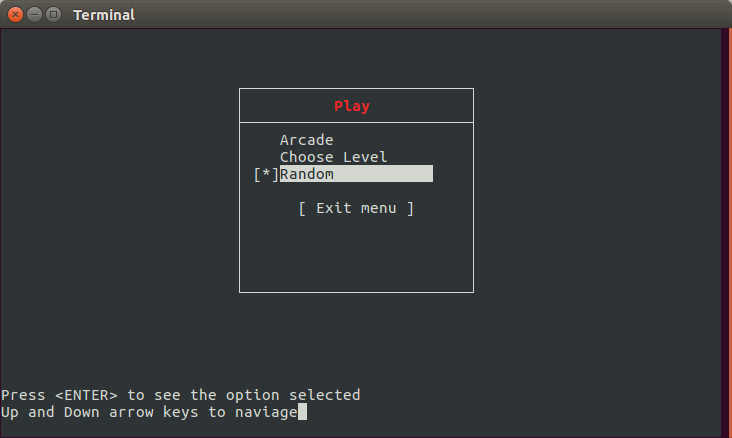
\includegraphics[width=0.75\textwidth]{annexe-manuel_utilisateur/rsrc/Menu_Play-random.png}
\end{center}

Dans ce menu, l'opérateur choisit le mode de jeu qu'il souhaite exploiter :
\begin{itemize}
	\item \textbf{Arcade :} Mode de jeu de type "time attack" dans lequel l'utilisateur doit résoudre des labyrinthes dans un temps imparti. Son score dépend du temps passé sur chaque labyrinthe et le nombre de déplacements qui lui ont été nécessaires pour sortir par rapport au nombre de déplacements nécessaires sur le chemin le plus court. Les dix meilleurs scores sont conservés en mémoire.
	\item \textbf{Choose level :} Mode de jeu dans lequel l'opérateur choisit entre cinq grilles prédéfinies chargées à partir d'un fichier.
	\item \textbf{Random :} Mode de jeu dans lequel une grille aléatoire est générée au lancement de la partie.
\end{itemize}

\paragraph{Nota :} Le mode de jeu "Arcade" n'est actuellement pas implémenté.

\paragraph{}La navigation dans ce menu est identique à celle du menu principal (touches directionnelles pour naviguer et touche "Entrée" pour valider).


\section{Menu "Choose level" - Choix d'une grille statique}

\begin{center}
	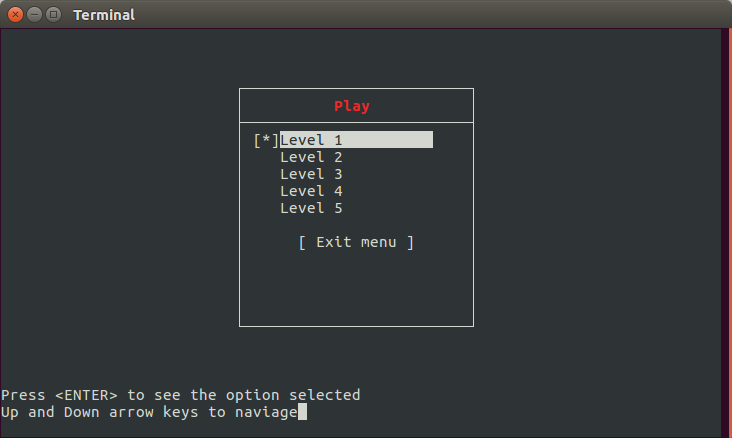
\includegraphics[width=0.75\textwidth]{annexe-manuel_utilisateur/rsrc/Menu_Play-grilles.png}
\end{center}

Ce menu apparaît lorsque l'opérateur sélectionne l'option \verb|"Choose level"| dans le menu \verb|"Play"|.

\paragraph{}L'opérateur peut choisir ici l'une des cinq grilles statiques inclues dans le jeu.

\paragraph{}La navigation dans ce menu est identique à celle du menu principal (touches directionnelles pour naviguer et touche "Entrée" pour valider).

\section{Gameplay}

Ci-après une capture d'écran d'un début de partie :
\begin{center}
	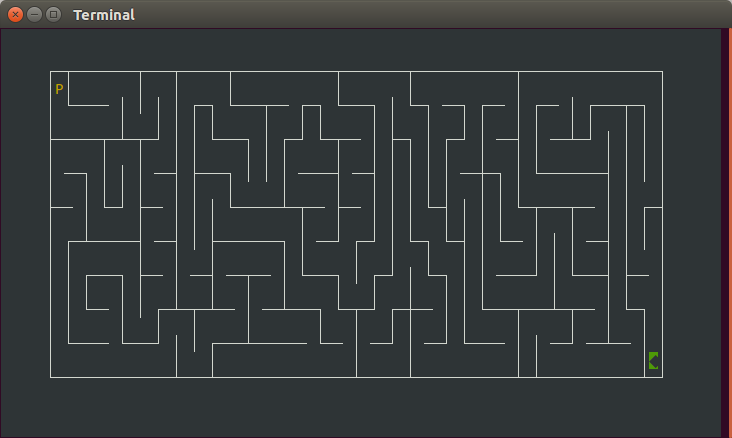
\includegraphics[width=0.75\textwidth]{annexe-manuel_utilisateur/rsrc/Labyrinthe-Debut.png}
\end{center}

La position du joueur est représentée par la lettre P clignotante, initialement située en haut à gauche de la grille.

La position de la sortie est représentée par le losange sur fond vert en bas à droite de l'écran.

Le but du jeu est pour le joueur de se déplacer dans le labyrinthe au moyen des touches directionnelles de son clavier dans le but d'atteindre la sortie.

Le chemin emprunté par le joueur ("fil d'Ariane") est représenté par de petits points au fur et à mesure de son avancée :
\begin{center}
	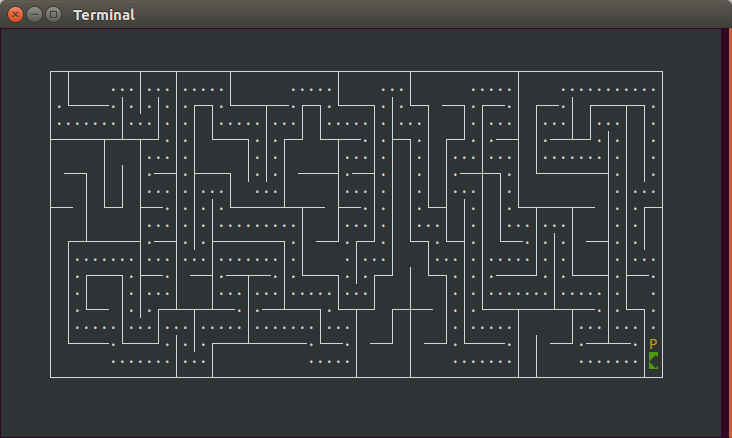
\includegraphics[width=0.75\textwidth]{annexe-manuel_utilisateur/rsrc/Labyrinthe-fin.png}
\end{center}

Une fois la partie terminée, une pop-up apparaît et le dernier menu utilisé ré-apparaît.